\documentclass[preprint,12pt,authoryear]{elsarticle}

\usepackage{amsmath,amssymb}
\usepackage{graphicx}
\usepackage{booktabs}
\usepackage[hidelinks]{hyperref}
\usepackage{xurl}

\journal{International Journal of Forecasting}

\begin{document}

\begin{frontmatter}

\title{Separating national and state-level predictability: a pre-registered forecast of Nigeria's \S134 presidential spread rule}

\author[inst1]{Anonymous Author}
\affiliation[inst1]{organization={Institution}}

\begin{abstract}
Several constitutions require a presidential winner to reach a vote threshold in enough subnational units; Nigeria's \S134 requires 25\% in two-thirds of the 36 states and the Federal Capital Territory. Forecasting such an event requires the joint distribution of the vote across units. We assemble a state-level dataset of Nigerian presidential results for 1999--2023 reconciled to official national totals, code \S134 under competing legal readings, and evaluate Bayesian models of the incumbent party's state vote share in leave-future-out backtests on 2015, 2019 and 2023, combined by prequential stacking. Given the true national vote, the stack lowers the state-level continuous ranked probability score by 10\% relative to the protocol's null swing model, better in two elections and tied in the third, but a zone-clustered bootstrap cannot exclude no difference. With the national vote forecast as well, no model beats simple baselines: the national forecast is no better than predicting no change, and most of the incumbent party's 19-point fall in 2023 coincided with opposition fragmentation. Unit-level intervals were too wide while the count of units above 25\% was too narrow and, in 2023, biased by an over-predicted regional realignment. A simulation study shows how little three elections can reveal. Two pre-registered 2027 forecasts, the second adding shared regional shocks, provide the out-of-sample test.
\end{abstract}

\begin{keyword}
election forecasting \sep proper scoring rules \sep forecast combination \sep pre-registration \sep multivariate evaluation \sep Nigeria
\end{keyword}

\end{frontmatter}

\section{Introduction}
\label{sec:intro}
Forecasting presidential elections in data-poor democracies is difficult and rarely evaluated with the rigour now standard in data-rich settings. In Nigeria, pre-election opinion polls have been criticised for weak methodology \citep{Mohammed2024OpinionPolls}, a qualitative reassessment of forecasts of the 2023 election found that conventional methods performed unevenly \citep{Murana2026RevisitingConventional}, and social-media signals have not proved a reliable substitute for polling \citep{Brito2021SystematicReview}. Public discussion therefore relies largely on expert judgement, whose accuracy is limited when it is not disciplined by explicit models and scoring \citep{Tetlock2006ExpertPolitical}.

Nigeria also illustrates a forecasting problem that is not specific to it. Section 134 of the 1999 Constitution \citep{Constitution1999} requires a winning candidate to obtain both the largest number of votes nationally and at least one-quarter of the votes cast in at least two-thirds of all the states and the Federal Capital Territory (FCT); otherwise a second, and possibly a third, election follows. Kenya requires an absolute national majority together with 25\% in more than half of its 47 counties \citep{KenyaConstitution2010}, and Indonesia an absolute majority together with 20\% in more than half of its provinces \citep{IndonesiaConstitution1945}. Whether such a rule is met depends on the joint distribution of the vote across units: the number of units above a threshold is sensitive to the national level, to where the units near the threshold sit, and to how their errors co-move. A forecast of the national vote alone cannot answer the question, and unit-level forecasts that are each well calibrated can still give a badly calibrated count.

This paper asks how much of this problem is forecastable from the historical record. It makes five contributions. First, we build a state-level presidential results dataset for 1999--2023, reconciled to the Independent National Electoral Commission's (INEC) official national totals, with every source and check documented. Second, we implement \S134 in code, including its two legally contested points and the second- and third-election procedure, with alternative readings as sensitivity checks. Third, we evaluate a family of Bayesian models of the incumbent party's state vote share with leave-future-out backtests, proper univariate and multivariate scoring rules and prequential stacking, separating the predictability of the national vote from that of its distribution across states. Fourth, a simulation study calibrated to the fitted Nigerian parameters quantifies how much three elections can reveal about forecasting skill and about the calibration of threshold counts. Fifth, we issue two pre-registered forecasts of the 2027 election, publicly timestamped before election day, with decision rules for their evaluation fixed in advance \citep{Monogan2015ResearchPreregistration}.

The results are mostly negative, and we think the negative results are the useful ones. Given the true national vote, the state distribution is somewhat forecastable: the stacked model beats the protocol's null swing model and the swing baselines on average, clearly in 2019 and narrowly or not at all in 2015, by a margin that three elections cannot establish. The national vote is not forecastable from its own history. The threshold count was poorly calibrated, for two separable reasons that a univariate evaluation would have hidden. We separate throughout the results of record, produced under a protocol frozen before the final run, from exploratory analyses added afterwards, and we explain why the backtests are only partly out of sample (Section~\ref{sec:protocol}); only the 2027 forecasts are clean tests.

\section{Background and Related Work}
\label{sec:related_work}

\subsection{Election forecasting}
Dynamic Bayesian models that combine fundamentals with state polls are well established in the United States \citep{Linzer2012DynamicBayesian, Heidemanns2020UpdatedDynamic, Chen2022PollsContext}, building on the observation that outcomes are predictable from fundamentals long before polls settle \citep{Gelman1993WhyAmerican} and on multilevel regression and poststratification for state-level estimation \citep{Park2004BayesianMultilevel}. Fundamentals-based forecasts are more uncertain than their in-sample fit suggests \citep{LauderdaleLinzer2015}. Bayesian approaches have been extended to multiparty systems \citep{Stoetzer2018ForecastingElections} and to subnational elections with little polling \citep{Stoetzer2025ElectionForecasting}, and synthetic models combine structural and poll-based information across countries \citep{LewisBeck2015Synthetic}. These models depend on polling whose total survey error is often larger than reported margins of error suggest \citep{Shiranimehr2018DisentanglingBias}. In settings with few elections and no reliable polls, simple models can be hard to beat \citep{Dawes1979RobustBeauty}. Related work has used past results to project partial returns in African elections \citep{Fridy2016ElectoralPredictions} and has forecast national elections with few past elections, as in Brazil \citep{Bertholini2022AgainstAll}.

\subsection{Uniform swing and reconciliation}
Uniform swing projects the national change in a party's vote onto every subnational unit; its assumptions materially shape district-level projections \citep{Erfort2026HowSwing}. Applied additively in percentage points it can leave the unit interval; applied on the logit scale it does not reproduce the national share it is given. Reconciling unit-level predictions with an aggregate by a common shift on the logit scale, the ``logit shift'', approximates a posterior update \citep{Rosenman2021RecalibrationPredictive}. We use it in the models and score both reconciled and unreconciled versions of the swing baselines.

\subsection{Combining and evaluating density forecasts}
Combinations of forecasts often beat their components, and simple combinations are hard to beat when weights must be estimated from few observations \citep{Claeskens2016Puzzle, Wang2023Combination}. For density forecasts, linear pools with weights chosen by the log score \citep{HallMitchell2007, GewekeAmisano2011} and stacking of Bayesian predictive distributions \citep{Yao2018UsingStacking} are standard; applied prequentially, so that the weights for each election use only earlier elections, the combination stays out of sample. Proper scoring rules, in particular the continuous ranked probability score (CRPS), assess calibration and sharpness jointly \citep{Gneiting2007StrictlyProper, Matheson1976ScoringRules, Gneiting2007Sharpness, Jordan2019EvaluatingProbabilistic}. Threshold counts depend on dependence between units, which univariate scores ignore; the energy score \citep{Gneiting2008Multivariate} and the variogram score \citep{ScheuererHamill2015} are sensitive to it. Comparisons of predictive accuracy need standard errors \citep{DieboldMariano1995}, but presidential elections are rare and state outcomes within an election are strongly correlated, so empirical evaluation has little power \citep{Grimmer2024AssessingReliability}.

\subsection{Regional voting in Nigeria}
African electoral competition is often organised around regional cleavages rooted in spatial inequality \citep{Boone2024InequalityPolitical, Boone2019RegionalInequalities}. In Nigeria, the homogeneity of voter choice in Fourth Republic presidential elections moved from a random spatial pattern in 1999 to a clustered one afterwards \citep{Nwankwo2019SpatialPattern}, and ethno-religious, regional and party affiliations continued to shape presidential vote choice in 2023 \citep{Abdulrazaq2024VotingPattern}. Spatial econometrics offers a framework for such dependence \citep{Lesage2009IntroductionSpatial}, but the weight matrix must usually be specified in advance \citep{Merk2021EstimationSpatial, Tan2024ParameterizingSpatial}. We test one pre-specified spatial structure, based on Nigeria's six geopolitical zones, against explicit candidate-region covariates, and explore shared zone shocks.

\section{Data}
\label{sec:data}

\subsection{State-level presidential results, 1999--2023}
We assembled presidential results for the 36 states and the FCT for 1999, 2003, 2011, 2015, 2019 and 2023 (Table~\ref{tab:election_results}). The 1999 results come from an IFES table of INEC data \citep{IFES1999}, the 2003 and 2011 results from archived INEC results websites \citep{INEC2003, INEC2011}, and the 2015 results from INEC's summary sheet \citep{INEC2015}. For 2019 and 2023, state results were announced at the national collation centre and images of the collation forms exist, but the INEC documents we could retrieve (the declarations of results and the post-election reports) give national figures only; we therefore take state party votes from Stears \citep{Stears2023} and registered voters from INEC's 2023 election report \citep{INEC2024Report}. The 1999 and 2015 sources are scanned documents read with optical character recognition; values were accepted only when arithmetic identities held (party votes summing to valid votes, and for 2015 valid plus rejected votes equalling votes cast). Four 1999 cells misread by OCR were corrected as the unique values satisfying those identities. 2007 is excluded: a 2018 press investigation reported that INEC holds no full official state-by-state breakdown of that result \citep{TheCable2018}, and we could locate national figures only.

For every year, the state votes of the leading parties sum to INEC's official national totals; in 2023, for example, the All Progressives Congress (APC) received 8,794,726 votes, the Peoples Democratic Party (PDP) 6,984,520, the Labour Party (LP) 6,101,533 and the New Nigeria Peoples Party (NNPP) 1,496,687. The remaining discrepancies and gaps are as follows. In 2011 the state sum for the Action Congress of Nigeria is 11,850 votes below INEC's national figure, and the 2011 valid-vote totals are sums of the party rows because INEC's file gives no valid-vote column. One 2015 cell differs by one vote from the printed column total. The archived 2003 Imo page reports 26 of 27 local government areas. For 2019 the ``others'' votes are derived as valid votes minus the two named parties, because the source's own ``others'' field (856,641 nationally) disagrees with its state totals (869,758). The 2019 and 2023 state figures reconcile to INEC's national party totals but cannot be checked against an INEC state table.

\begin{table}[ht]
\centering
\caption{Curated state-level presidential results. ``Parties recorded'' is the number of parties with separate state-level vote counts in the source; remaining parties are grouped as ``others'' (2019 had 73 candidates).}
\label{tab:election_results}
\begin{tabular}{lrrr}
\toprule
Year & Units & Parties recorded & Total valid votes \\
\midrule
1999 & 37 & 2 & 29,848,441 \\
2003 & 37 & 20 & 39,480,489 \\
2011 & 37 & 20 & 38,199,219 \\
2015 & 37 & 14 & 28,587,564 \\
2019 & 37 & 2 & 27,324,583 \\
2023 & 37 & 4 & 24,025,940 \\
\bottomrule
\end{tabular}
\end{table}

\subsection{Target}
The target is the incumbent (ruling) party's share of valid votes in each state: the PDP from 2003 to 2015 and the APC from 2019 to 2027. The 1999 election, which ended military rule, has no incumbent party and serves only as the lag for 2003. Because 2007 is missing, 2011 is lagged against 2003, a transition spanning eight years and a change of president that is treated like the four-year transitions. Defining the target by incumbency pools two parties across the 2015 change of government; the 2019 lag is the APC's own 2015 share, so each transition compares the same party, and the models' state terms describe how a state's position relative to the national incumbent vote evolves.

Table~\ref{tab:national} shows the national series with two measures of the structure of competition: the incumbent party's share of the top-two vote and the effective number of parties by votes \citep{Laakso1979ENP}, computed over the parties recorded by name (votes for unrecorded parties are treated as fully fragmented, which slightly overstates the effective number in years with few named parties). Arithmetically, the 19-point fall of 2023 coincided with a rise in the effective number of parties from 2.1 to 3.5 and a fall of only 1.7 points in the incumbent's two-party share; this is a decomposition, not a causal claim.

\begin{table}[ht]
\centering
\caption{Incumbent-party national share of valid votes, its share of the top-two vote, and the effective number of parties (ENP, by votes, over parties recorded by name).}
\label{tab:national}
\small
\setlength{\tabcolsep}{4pt}
\begin{tabular}{lllrrcrr}
\toprule
Election & Party & Lag & Share & Lagged & Pres.\ running & Two-party & ENP \\
\midrule
2003 & PDP & 1999 & 0.619 & 0.628 & yes & 0.658 & 2.05 \\
2011 & PDP & 2003 & 0.589 & 0.619 & yes & 0.648 & 2.21 \\
2015 & PDP & 2011 & 0.450 & 0.589 & yes & 0.455 & 2.03 \\
2019 & APC & 2015 & 0.556 & 0.540 & yes & 0.574 & 2.09 \\
2023 & APC & 2019 & 0.366 & 0.556 & no & 0.557 & 3.49 \\
2027 & APC & 2023 & -- & 0.366 & yes & -- & -- \\
\bottomrule
\end{tabular}
\end{table}

\subsection{Covariates}
All covariates are measured before election day.
\begin{itemize}
\item \textbf{Candidate home state and zone.} Indicators for whether a state is the home state, or in the home geopolitical zone, of the incumbent party's candidate, and whether it is in the home zone of a major challenger, for the current and the previous election. Home states were coded from public candidate information; the coding is in the replication files.
\item \textbf{North/South region.} Indicators for whether a state lies in the region (North: North-Central including the FCT, North-East, North-West; South: South-East, South-South, South-West) of the incumbent party's candidate and of the main challenger, current and lagged. The main challenger is the major opposition party listed first by its previous-election strength, which is known before the election.
\item \textbf{Political violence.} Events and fatalities from ACLED \citep{Raleigh2010IntroducingAcled, ACLEDHDX} in the 12 full months before the election month, combined as $\log(1+\text{events})+\log(1+\text{fatalities})$ and standardised within each election year to remove ACLED's growing coverage over time.
\end{itemize}
State poverty estimates \citep{OPHIMPI} exist only from 2013 and are excluded. National macroeconomic indicators cannot explain state deviations and, with at most five national observations, are not used in the national model.

\section{Methodology}
\label{sec:method}

\subsection{The \S134 rule}
Under \S134(2), a candidate is elected outright with the highest number of votes nationally and at least 25\% of the votes in each of at least two-thirds of all the states and the FCT \citep{Constitution1999}. Following the Supreme Court's 2023 decisions \citep{ObiINEC2023}, the FCT is treated as one of 37 units, so two-thirds is $24\tfrac{2}{3}$ units. Following \textit{Awolowo v. Shagari} \citep{AwolowoShagari1979}, in which two-thirds of 19 states was held to be $12\tfrac{2}{3}$ states, the fraction is met by 25\% in 24 units plus at least two-thirds of 25\% (16.67\%) in a 25th. We report three alternative readings: two-thirds of the 36 states only; 24 states plus 25\% in the FCT (the petitioners' reading rejected in 2023); and 25 whole units. If no candidate is elected, \S134(3)--(5) require a second election within seven days between the national leader and the remaining candidate with a majority of votes in the highest number of states, and, failing a winner with a majority and the same spread, a third election decided by simple majority.

\subsection{Model}
Let $y_{it}$ be the incumbent party's share in state $i$ at election $t$ and $N_t$ its national share. We decompose $\operatorname{logit} y_{it} = \operatorname{logit} N_t + d_{it}$, where $d_{it}$ is the state deviation. All candidate models share one national model,
\begin{equation}
\operatorname{logit} N_t - \operatorname{logit} N_{t-1} = \mu + \gamma\, r_t + e_t, \qquad e_t \sim \mathcal{N}(0, \sigma_n^2),
\end{equation}
where $r_t$ indicates that the incumbent party's candidate is the sitting president, with priors $\mu, \gamma \sim \mathcal{N}(0, 0.5^2)$ and $\sigma_n \sim \text{HalfNormal}(0.5)$. In every backtest all training swings have $r_t = 1$, so only $\mu + \gamma$ is identified by the data and the 2023 backtest forecast, the only one with $r_t = 0$, depends on how the prior divides that sum; in the 2027 fit $\gamma$ is identified by the single 2023 observation. State deviations follow either a level model,
\begin{equation}
d_t = \alpha + \phi\, d_{t-1} + X_t \beta + u + \varepsilon_t,
\end{equation}
or a swing model, which fixes $\phi = 1$, optionally with a spatial autoregressive filter on the change in deviations,
\begin{equation}
(I - \rho W)(d_t - d_{t-1}) = \alpha + X_t \beta + u + \varepsilon_t ,
\end{equation}
so that in the swing model $u_i$ is a state-specific drift rather than a level. $W$ is a row-standardised zone-block matrix linking states in the same geopolitical zone, $u_i \sim \mathcal{N}(0, \tau^2)$ and $\varepsilon_t \sim \mathcal{N}(0, \sigma^2 I)$. Priors are $\rho \sim \text{Uniform}(-1,1)$, $\beta, \alpha \sim \mathcal{N}(0, 0.5^2)$, $\tau \sim \text{HalfNormal}(0.3)$ and $\sigma \sim \text{HalfNormal}(0.5)$. The spatial likelihood is exact, with the log-determinant from the eigenvalues of $W$. Conditional on the national draw, the non-spatial models treat states as independent.

Predictions draw a national swing and a vector of state deviations from the posterior predictive distribution; each draw's state logits are then shifted by a common constant so that the vote-weighted mean of the state shares equals the national draw (the logit shift; \citealp{Rosenman2021RecalibrationPredictive}). The weights are each state's share of valid votes at the previous election, because current turnout is unknown before the election; applied to the actual results, these lagged weights reproduce the national share to within 1.0, 2.9 and 0.5 percentage points in 2015, 2019 and 2023. Point forecasts are posterior medians. Models are estimated in PyMC \citep{AbrilPla2023PyMC} with the No-U-Turn sampler \citep{Hoffman2011NouturnSampler}, four chains of 1,000 draws after 1,000 tuning steps, and a target acceptance rate of 0.99. Simulation-based calibration of the national model and the dominant state model is reported in Appendix~\ref{app:sbc}.

\subsection{Candidate models and baselines}
The protocol fixes six candidates: \texttt{ps\_null} (swing model with intercept, state drift and noise, no covariates); \texttt{ps\_home} (swing model with home-state, home-zone and violence covariates); \texttt{ps\_region} (adds the North/South region covariates); \texttt{sar\_region} (\texttt{ps\_region} with the spatial filter); \texttt{pp\_region} (level model with region covariates and a persistence prior $\phi \sim \mathcal{N}(1, 0.2^2)$); and \texttt{lvl\_home} (level model with $\phi \sim \mathcal{N}(0,1)$, kept as a reference). The protocol's comparators are \texttt{ps\_null}, logit uniform swing (not reconciled) and persistence.

Because unreconciled baselines do not reproduce the national share they are given, we added, after review, reconciled and additive versions: additive uniform swing (percentage points, clipped to the unit interval), reconciled logit uniform swing, and probabilistic uniform swing (PUS), which centres each state on logit uniform swing and adds Gaussian noise whose standard deviation is the root mean square of uniform-swing residuals in the training elections (1.99, 1.67 and 1.56 on the logit scale for the three backtests), with and without reconciliation. In forecast mode the swing baselines receive the national model's predictive draws. Deterministic baselines given the true national share have no predictive spread, and their CRPS equals their mean absolute error.

\subsection{Prequential stacking}
For each target election $t$, every candidate is fitted on elections before $t$, and the stacking weights for $t$ maximise $\sum_i \log \sum_k w_k\, p_k(y_i)$ over held-out state outcomes from backtests of earlier targets only \citep{Yao2018UsingStacking}: equal weights for 2015, the 37 outcomes of the 2015 backtest for 2019, 74 outcomes for 2023 and 111 for the 2027 forecast. Predictive densities are approximated by Gaussians on the logit scale and evaluated in oracle mode. The stacked predictive distribution is the weighted mixture of the candidates' draws, which adds Monte Carlo error with a standard deviation of 0.02--0.09 percentage points to the stack's CRPS in each election (less for the three-election mean); the baselines' simulated noise adds similar error. The criterion is a sum of marginal log densities, so it cannot reward a model for getting the dependence between states right. Appendix~\ref{app:weights} reports the weights' robustness and sampling uncertainty.

\subsection{Evaluation protocol, development history and its limits}
\label{sec:protocol}
Backtests train on elections before $t$ and predict $t \in \{2015, 2019, 2023\}$; the 2015 backtest has only two training elections. Every model is scored in forecast mode, with the shared national model's forecast, and in oracle mode, with the true national share, which isolates state-level skill. The protocol's primary metric is the mean state-level CRPS in percentage points; secondary metrics are the RMSE and MAE of the posterior median (averaged over elections), 90\% interval coverage, the Brier score for each state's 25\% event, the national error and the probability that the \S134 spread is met. After review we added the energy score over the 37 units (in percentage points), the variogram score of order 0.5, the ranked probability score (RPS) of the count of units at 25\%, interval width and probability integral transform (PIT) histograms.

We disclose the development history in full. A first version (v1a) used level models only. Its persistence parameter was estimated at 0.13--0.52 across backtests (in the 2015 backtest identified from just the 1999--2003 and 2003--2011 transitions); the level models beat uniform swing in oracle mode (mean CRPS 10.61 and 10.66 for the non-spatial and spatial versions against 11.05) but were far worse in forecast mode (13.07 and 13.06 against 10.96). Swing models were added after seeing these results. We then wrote an evaluation protocol (v2) fixing the six candidates, one new covariate family (North/South region), the stacking procedure and the metrics; its hash is recorded with every result file. One change was made afterwards: divergent transitions in the first v2 run (26 in the 2015 national fit, which has two observations) led us to raise the sampler's target acceptance rate from 0.95 to 0.99; both runs are archived and the results were essentially unchanged.

The freeze is self-attested. The protocol and the v2 results were first committed together, so the record shows that the results correspond to the protocol text but not that the text preceded the run. The protocol was written after the v1 results were seen, and the North/South covariate was chosen by an author who knew how 2015, 2019 and 2023 turned out. We therefore describe the backtests as partly out of sample. Only the 2027 forecasts, made public before the election, are clean tests. Everything added after the v2 run, including all reconciled and additive baselines, multivariate scores, bootstraps, the zone-shock models, the simulation study and the sensitivity analyses, is labelled exploratory and changes neither the result of record nor the primary 2027 forecast.

\section{Evaluation Results}
\label{sec:experiments}

\subsection{State-level skill given the national vote}
Table~\ref{tab:results_oracle} reports mean oracle-mode performance. Among the protocol's models and comparators, the prequential stack has the lowest CRPS, 7.86 percentage points, against 8.77 for \texttt{ps\_null} (10\% lower) and 11.05 for logit uniform swing. The comparison with uniform swing mostly rewards having any predictive spread, since a deterministic forecast's CRPS equals its absolute error. Reconciling or re-scaling the baselines changes little: the reconciled PUS scores 8.99 and the reconciled and additive uniform swings 11.01 and 11.44. The stack's median is also the most accurate point forecast among these (RMSE 12.62 against 14.11--15.26 for the baselines), and its energy score (57.8) and variogram score (1,937 against 2,097--2,438) are the lowest among the protocol's models and comparators; because the energy score is dominated by the marginals, the variogram score is the better indication that the gain extends to the joint distribution. On the count of units at 25\%, however, the stack's RPS (3.54) is worse than that of \texttt{pp\_region} (2.95) and \texttt{lvl\_home} (3.20).

\begin{table}[ht]
\centering
\caption{Mean backtest performance over 2015, 2019 and 2023, \textbf{oracle mode} (true national share supplied). CRPS, RMSE, interval width and energy score in percentage points; RPS of the count of units at 25\%. US: uniform swing; PUS: probabilistic uniform swing. $^\dagger$ Exploratory: added after the v2 results were seen.}
\label{tab:results_oracle}
\small
\setlength{\tabcolsep}{3pt}
\begin{tabular}{lrrrrrr}
\toprule
Model & CRPS & RMSE & Cov.\ 90\% & Width & Energy & Count RPS \\
\midrule
stack & 7.86 & 12.62 & 0.95 & 66.2 & 57.8 & 3.54 \\
ps\_region & 8.29 & 15.06 & 0.99 & 62.6 & 58.6 & 5.54 \\
pp\_region & 8.33 & 14.06 & 0.95 & 62.1 & 61.6 & 2.95 \\
ps\_home & 8.71 & 15.48 & 0.99 & 64.2 & 60.0 & 5.96 \\
ps\_null & 8.77 & 14.95 & 0.99 & 70.4 & 59.9 & 6.29 \\
sar\_region & 8.88 & 15.34 & 1.00 & 71.9 & 62.1 & 5.31 \\
lvl\_home & 10.67 & 19.18 & 0.90 & 69.1 & 80.5 & 3.20 \\
US (logit) & 11.05 & 14.21 & 0.00 & 0.0 & 86.4 & 3.67 \\
\midrule
PUS, reconciled$^\dagger$ & 8.99 & 15.26 & 0.99 & 72.2 & 61.0 & 6.43 \\
PUS$^\dagger$ & 9.14 & 14.37 & 0.99 & 73.9 & 62.8 & 5.02 \\
US, reconciled$^\dagger$ & 11.01 & 14.15 & 0.00 & 0.0 & 86.1 & 5.33 \\
US, additive$^\dagger$ & 11.44 & 14.11 & 0.00 & 0.0 & 85.8 & 4.00 \\
stack, no region$^\dagger$ & 8.18 & 12.96 & 1.00 & 71.9 & 59.3 & 4.68 \\
pp\_region + zone shock$^\dagger$ & 7.41 & 11.98 & 0.97 & 62.6 & 55.1 & 2.96 \\
ps\_region + zone shock$^\dagger$ & 7.91 & 14.24 & 0.99 & 59.8 & 55.6 & 5.43 \\
\bottomrule
\end{tabular}
\end{table}

Three elections give little power. Table~\ref{tab:paired} reports the stack's CRPS minus that of the main comparators, election by election, with 90\% intervals from resampling the six geopolitical zones as blocks, which respects the regional clustering of errors (with six blocks these intervals are coarse). The stack is better than \texttt{ps\_null} and than the reconciled PUS in all three elections, but the gain is concentrated in 2019, the stack and \texttt{ps\_null} are tied in 2015, and the intervals for the three-election mean include zero. Against the reconciled uniform swing, the stack is better on average but not in 2015. The defensible statement is that the oracle-mode evidence is consistent with a modest state-level gain, not that it establishes one.

\begin{table}[ht]
\centering
\caption{Stack CRPS minus comparator CRPS (percentage points; negative favours the stack; US: uniform swing), with 90\% intervals from 2,000 resamples of the six geopolitical zones within each election. Exploratory.}
\label{tab:paired}
\footnotesize
\setlength{\tabcolsep}{3pt}
\begin{tabular}{llcccc}
\toprule
Mode & Comparator & 2015 & 2019 & 2023 & Mean \\
\midrule
oracle & ps\_null & $-0.04$ & $-2.10$ & $-0.58$ & $-0.91$ \\
 & & {\scriptsize [$-0.70$, 0.67]} & {\scriptsize [$-3.68$, $-0.60$]} & {\scriptsize [$-4.09$, 2.83]} & {\scriptsize [$-2.22$, 0.39]} \\
oracle & PUS, reconciled & $-0.43$ & $-2.15$ & $-0.81$ & $-1.13$ \\
 & & {\scriptsize [$-1.09$, 0.24]} & {\scriptsize [$-3.76$, $-0.68$]} & {\scriptsize [$-4.27$, 2.89]} & {\scriptsize [$-2.41$, 0.19]} \\
oracle & US, reconciled & 0.11 & $-5.00$ & $-4.55$ & $-3.15$ \\
 & & {\scriptsize [$-1.08$, 1.05]} & {\scriptsize [$-8.45$, $-2.04$]} & {\scriptsize [$-10.49$, 0.67]} & {\scriptsize [$-5.34$, $-1.11$]} \\
\midrule
forecast & ps\_null & 0.16 & $-1.40$ & 2.03 & 0.26 \\
 & & {\scriptsize [$-1.40$, 2.15]} & {\scriptsize [$-3.89$, 1.21]} & {\scriptsize [$-1.84$, 6.19]} & {\scriptsize [$-1.37$, 2.11]} \\
forecast & PUS, reconciled & $-0.10$ & $-1.53$ & 2.05 & 0.14 \\
 & & {\scriptsize [$-1.64$, 1.69]} & {\scriptsize [$-4.17$, 1.00]} & {\scriptsize [$-2.21$, 6.38]} & {\scriptsize [$-1.64$, 1.98]} \\
forecast & US, reconciled & $-0.16$ & $-0.24$ & 1.71 & 0.44 \\
 & & {\scriptsize [$-2.18$, 2.21]} & {\scriptsize [$-5.07$, 4.10]} & {\scriptsize [$-4.59$, 7.71]} & {\scriptsize [$-2.21$, 3.03]} \\
\bottomrule
\end{tabular}
\end{table}

\begin{figure}[ht]
\centering
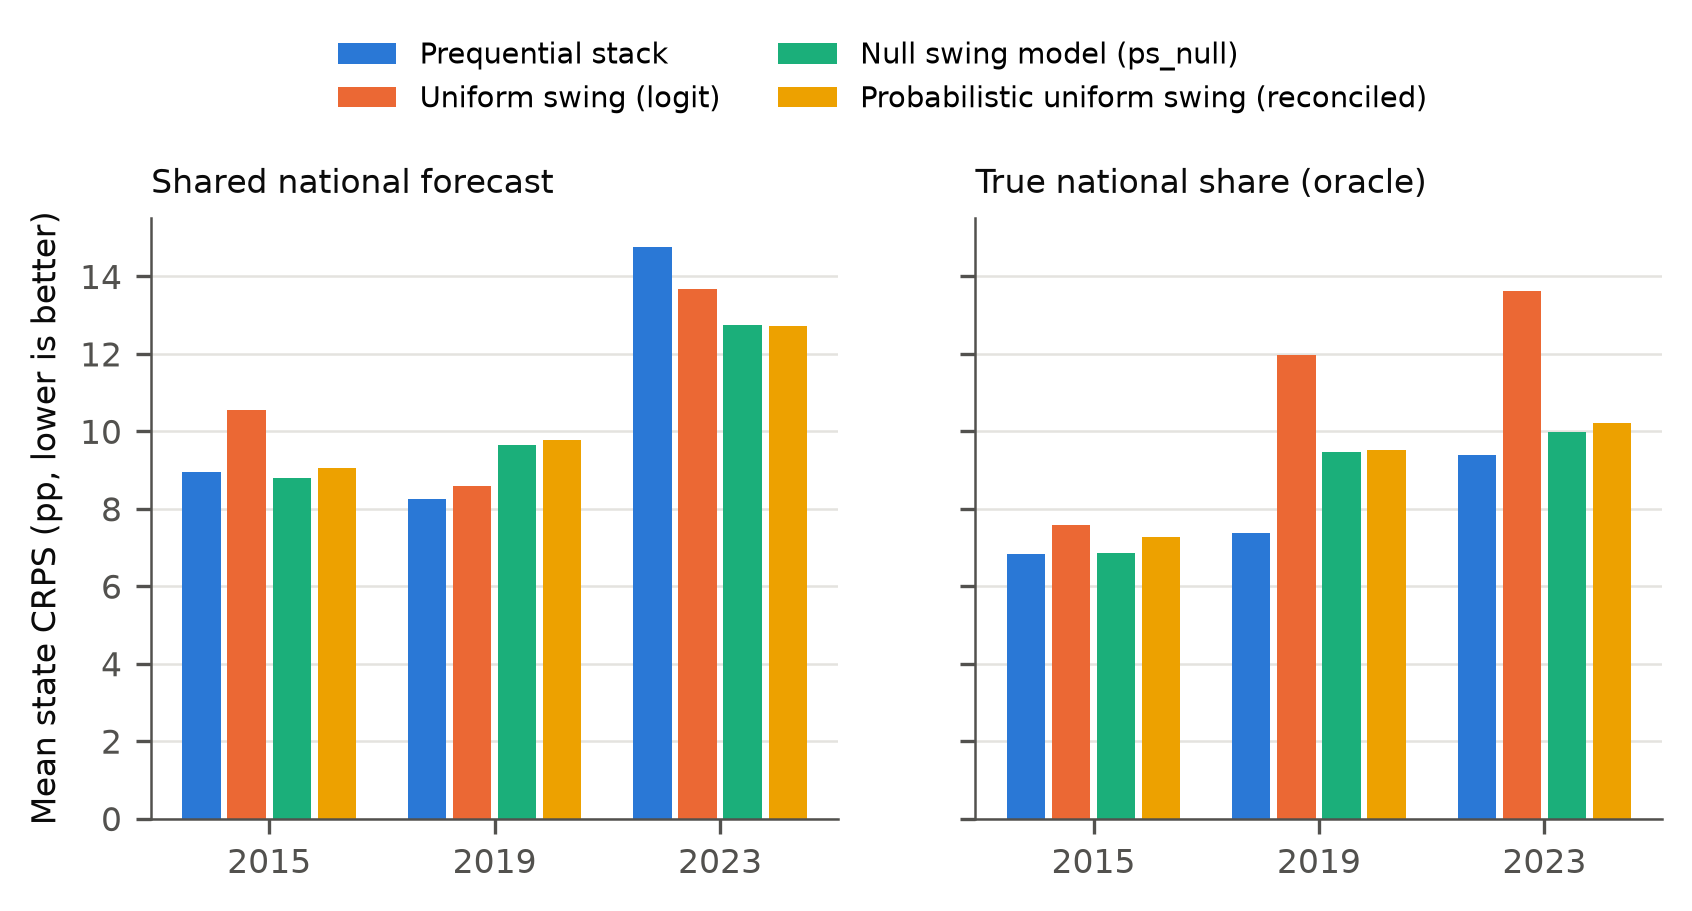
\includegraphics[width=\linewidth]{figures/fig1_backtest_crps.png}
\caption{Leave-future-out backtests: mean state-level CRPS (percentage points, lower is better) for 2015, 2019 and 2023: prequential stack, logit uniform swing, the null swing model (\texttt{ps\_null}) and reconciled probabilistic uniform swing (exploratory). Left: the shared national model's forecast is used, so all four have predictive spread. Right: the true national share is supplied (oracle), in which case uniform swing is deterministic.}
\label{fig:backtest_crps}
\end{figure}

\subsection{The national vote is not forecastable from its own history}
\label{sec:national}
In forecast mode, no protocol model reliably beats the baselines (Tables~\ref{tab:paired} and~\ref{tab:results_forecast}). The stack's CRPS is 10.66, against 10.39 for \texttt{ps\_null} and 10.16--10.93 for the uniform-swing variants, which in this mode all receive the national model's draws; additive uniform swing, added after review, has the lowest CRPS of all forecasts other than the exploratory zone-shock models. The shared national model forecast 0.569, 0.484 and 0.534 against outcomes of 0.450, 0.556 and 0.366, errors of $+11.9$, $-7.2$ and $+16.8$ percentage points. A naive forecast that the incumbent party repeats its previous share has errors of $+13.9$, $-1.6$ and $+19.0$: a slightly lower mean absolute error (11.5 against 12.0) and a higher RMSE (13.6 against 12.6). The national model adds nothing measurable to a no-change forecast, and its 90\% intervals contained all three outcomes only because they are wide.

\begin{table}[ht]
\centering
\caption{Mean backtest performance over 2015, 2019 and 2023, \textbf{forecast mode} (shared national model's forecast). Units as in Table~\ref{tab:results_oracle}. $^\dagger$ Exploratory.}
\label{tab:results_forecast}
\small
\setlength{\tabcolsep}{3pt}
\begin{tabular}{lrrrrrr}
\toprule
Model & CRPS & RMSE & Cov.\ 90\% & Width & Energy & Count RPS \\
\midrule
ps\_region & 10.34 & 17.61 & 0.95 & 71.2 & 72.5 & 3.52 \\
ps\_null & 10.39 & 16.64 & 0.99 & 77.4 & 71.1 & 3.73 \\
stack & 10.66 & 17.90 & 0.96 & 73.4 & 76.8 & 3.10 \\
ps\_home & 10.80 & 18.47 & 0.97 & 72.2 & 74.4 & 3.78 \\
sar\_region & 10.90 & 18.40 & 0.98 & 78.6 & 76.3 & 3.57 \\
US (logit) & 10.93 & 17.04 & 0.47 & 24.6 & 84.1 & 4.32 \\
pp\_region & 11.10 & 19.40 & 0.95 & 69.6 & 80.6 & 3.23 \\
lvl\_home & 13.09 & 23.98 & 0.91 & 75.4 & 96.8 & 3.33 \\
persistence & -- & 17.94 & -- & -- & -- & -- \\
\midrule
US, additive$^\dagger$ & 10.16 & 17.12 & 0.64 & 31.3 & 81.2 & 4.17 \\
US, reconciled$^\dagger$ & 10.22 & 16.82 & 0.68 & 34.9 & 78.7 & 4.10 \\
PUS$^\dagger$ & 10.48 & 17.08 & 0.99 & 76.0 & 72.1 & 3.96 \\
PUS, reconciled$^\dagger$ & 10.51 & 16.70 & 0.99 & 78.7 & 71.9 & 3.76 \\
stack, no region$^\dagger$ & 10.69 & 18.29 & 0.98 & 78.3 & 76.2 & 3.55 \\
pp\_region + zone shock$^\dagger$ & 9.94 & 16.98 & 0.95 & 70.5 & 72.9 & 3.32 \\
ps\_region + zone shock$^\dagger$ & 9.82 & 16.45 & 0.97 & 69.3 & 68.7 & 3.60 \\
\bottomrule
\end{tabular}
\end{table}

The national predictive distribution also depends on the priors. Because $\mu$ and $\gamma$ are identified only through their sum in the backtests, alternative priors change the backtest errors by less than 2 points but change the interval widths: under priors half as wide, the 2015 and 2023 outcomes fall outside the 90\% interval (Appendix~\ref{app:national}). The most important omission is the structure of competition. The 19-point fall in 2023 coincided with a rise in the effective number of parties from 2.1 to 3.5 and only a 1.7-point fall in the two-party share (Table~\ref{tab:national}). A model of vote share alone cannot anticipate such changes; forecasting them needs information about the candidate field that is not in the historical series.

\subsection{Why the ranking reverses between modes}
\label{sec:flip}
The stack is best in oracle mode but not in forecast mode, and in 2023 its forecast-mode RMSE (25.7) exceeds that of logit uniform swing (21.9). Each model's forecast-mode squared error equals its oracle-mode squared error, plus the squared shift that the national error induces in its state medians, plus twice their cross-product. The reconciled forecasts receive similar shifts, so rankings are decided largely by the cross term: whether a model's state errors given the true national share happen to offset or compound the national error. In 2023 the national share was over-forecast by 17 points. The stack's oracle-mode errors were regional (northern states under-predicted by 7.9 points on average, southern states over-predicted by 9.0), so in forecast mode its southern errors compounded to $+28.0$ points, whereas \texttt{ps\_null}, which under-predicted most states in oracle mode, was partly rescued by the national over-forecast (cross term $-306$ against $-11$ for the stack, in squared percentage points).

Whether such reversals indicate anything systematic is a question about power, which the simulation study in Appendix~\ref{app:simulation} addresses. In a synthetic country calibrated to the fitted Nigerian parameters, national forecast errors of the Nigerian size (0.48, 0.29 and 0.69 on the logit scale in the three backtests) shrink a genuine state-level advantage in forecast mode by roughly 15--35\% but do not reverse it on average: the better model ranks first in forecast mode about as often as in oracle mode. What limits power is the number of elections. With three elections, a model whose true state-level advantage is about 0.5 CRPS points is ranked first only about 80\% of the time, and one with an advantage of about 0.13 points only about 70\% of the time. The Nigerian forecast-mode reversal is therefore consistent with chance. The observed oracle-mode gain over \texttt{ps\_null} (0.91 points) lies between the simulated cells in which the better model ranks first 81--98\% of the time, so three elections would usually, but not reliably, detect a gain of this size, and would rarely detect the smaller gains among the candidate models.

\subsection{Spatial dependence, regional covariates and stacking weights}
The spatial term did not improve forecasts: \texttt{sar\_region} scored worse than the otherwise identical \texttt{ps\_region} (oracle CRPS 8.88 against 8.29) although its spatial parameter was substantial ($\rho$ 0.62--0.64), and it received zero weight in the 2019 and 2023 stacks and in the 2027 weights. The result concerns one weight matrix, which links every state in a zone equally and so behaves much like a zone effect on the swing, and a stacking criterion that cannot reward dependence. Its count calibration was no better than that of the non-spatial models (Appendix~\ref{app:count}).

The North/South region family improved on home-zone covariates on average (oracle CRPS 8.29 against 8.71), and the stack built without it scores 8.18 in oracle mode and 10.69 in forecast mode, against 7.86 and 10.66. But the gain comes from 2015 and 2019, which the author had seen when choosing the covariate. In 2023, the only election in which the incumbent party's candidate switched region, \texttt{ps\_region} scored worse than \texttt{ps\_home} (9.98 against 9.83) and the zero-weight \texttt{lvl\_home} was best (8.70). The incumbent candidate's region effect cannot be separated from its lag in any of the three backtests, because the candidate never switched region within a training window, so it is identified only by the prior; in the 2027 fit it is identified by the single 2023 switch. The main challenger's home-region coefficient was negative throughout, for example $-0.75$ (posterior s.d.\ 0.22) in \texttt{ps\_region} fitted for 2023.

The stacking weights (Table~\ref{tab:weights}) moved from equal weights in 2015 to \texttt{pp\_region} (0.70) and \texttt{ps\_region} (0.30) in 2019, and to \texttt{pp\_region} alone in 2023, so the 2023 stack is effectively model selection. Resampling states, the 90\% interval for \texttt{pp\_region}'s weight is $[0.06, 1.00]$ for 2019 and $[0.56, 1.00]$ for 2027 (Appendix~\ref{app:weights}). The posterior persistence in \texttt{pp\_region} was 0.31, 0.41 and 0.49 in the three training windows, so the data favour substantial mean reversion of state deviations given the candidate-region terms.

\begin{table}[ht]
\centering
\caption{Prequential stacking weights (result of record). Each column uses backtests of earlier targets only; the last column is used for 2027.}
\label{tab:weights}
\begin{tabular}{lrrrr}
\toprule
Model & 2015 & 2019 & 2023 & 2027 \\
\midrule
ps\_null & 0.167 & 0.000 & 0.000 & 0.000 \\
ps\_home & 0.167 & 0.000 & 0.000 & 0.000 \\
ps\_region & 0.167 & 0.300 & 0.000 & 0.188 \\
sar\_region & 0.167 & 0.000 & 0.000 & 0.000 \\
pp\_region & 0.167 & 0.700 & 1.000 & 0.812 \\
lvl\_home & 0.167 & 0.000 & 0.000 & 0.000 \\
\bottomrule
\end{tabular}
\end{table}

\subsection{Calibration, the threshold count and the \S134 spread}
The stack's state-level 90\% intervals covered 100\%, 100\% and 86\% of outcomes in 2015, 2019 and 2023, with a mean width of 66 percentage points in oracle mode, and the pooled PIT histograms are hump-shaped (Appendix~\ref{app:count}): the unit-level predictive distributions are too wide. Yet the predictive distribution of the \emph{number} of units at 25\% was too narrow. Its standard deviation was about two units (1.6--2.6) for every candidate in oracle mode, and the outcomes (26, 34 and 29 units) fell at the 83rd, 98th and 99.9th percentiles of the stack's distribution (Figure~\ref{fig:spread_count}). Treating states as conditionally independent contributes, because independent errors largely cancel in the count, but it is not the main cause: adding shared zone shocks widens the count distribution only from about 2.1 to 2.8 units, and the outcomes remain in its upper tail (Appendix~\ref{app:count}). The main cause is location, as the next paragraph shows. For the state-level 25\% event, Brier skill scores relative to each state's historical frequency range from 0.29 to 0.42 across candidates (stack 0.39; \texttt{pp\_region} 0.42).

The incumbent party met the \S134 spread in all three elections, but the stack's oracle-mode probability was 0.462, 0.985 and 0.379; deterministic uniform swing, given the true national share, predicted it correctly every time. In all three years the count was under-predicted mainly because states near the threshold were placed on the wrong side of it. In 2015 two states that reached 25\% (Kaduna and Osun) had medians below it. In 2019, when the spread probability was high, the count shortfall (median 29 against 34 units) came from four southern states (Abia, Bayelsa, Delta and Ebonyi) with medians below 25\%. In 2023 the miss was a regional bias rather than a dispersion problem: the stack's medians were \emph{less} dispersed than the outcomes (standard deviation of logit medians 0.86 against 1.26), but all seven states that reached 25\% while the stack's median was below it were northern (Jigawa, Kaduna, Kebbi, Kano, Katsina, Sokoto and Zamfara). The model anticipated a larger North-to-South realignment, following the incumbent party's switch to a southern candidate, than occurred. Excess width also contributes where medians lie close to the threshold. Narrowing each state's predictive distribution about its median by a factor chosen on earlier backtests (0.39 for 2019, 0.42 for 2023) raises the 2019 probability to 1.00 and lowers the mean oracle CRPS from 7.86 to 7.66 (2019: 7.36 to 6.29), but worsens 2023 (9.39 to 9.85), raises the 2023 probability only to 0.63, and cuts coverage to 84\% and 68\%. Three ``met'' outcomes carry little information about the calibration of this event, and in 2015 the incumbent lost, so the event had no legal consequence.

\begin{figure}[ht]
\centering
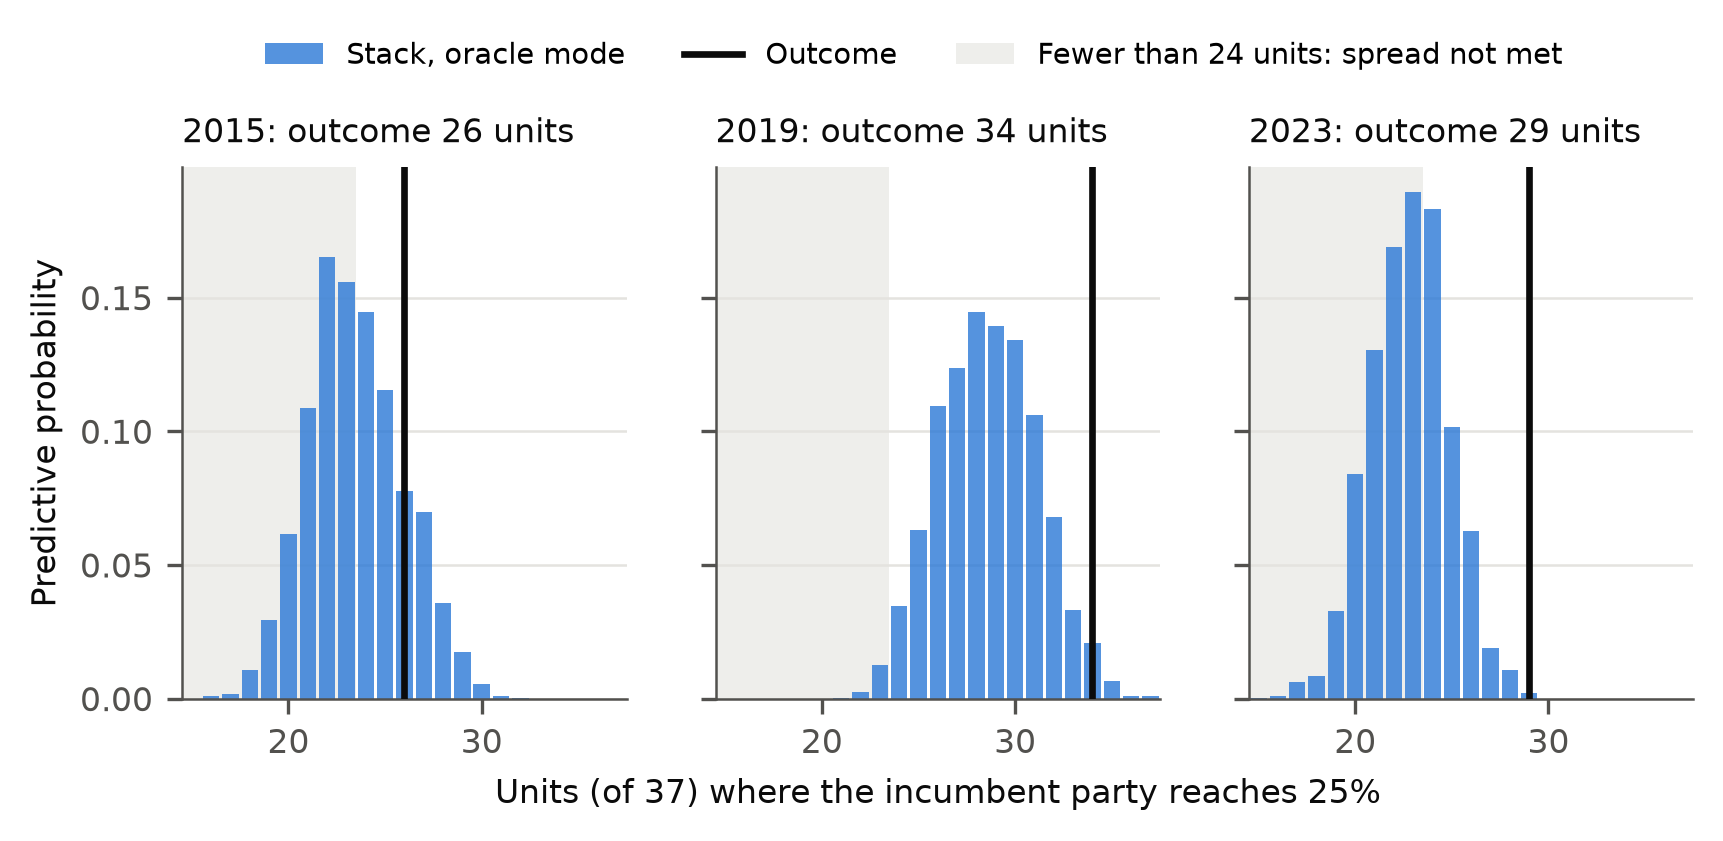
\includegraphics[width=\linewidth]{figures/fig5_spread_count.png}
\caption{Predictive distribution of the number of units (of 37) in which the incumbent party reaches 25\%, prequential stack in oracle mode, against the outcome (black line). The \S134 spread requires 25\% in 24 units plus 16.67\% in a 25th, so it cannot be met with fewer than 24 units (shaded) and is met with 25 or more. Exploratory.}
\label{fig:spread_count}
\end{figure}

\begin{figure}[ht]
\centering
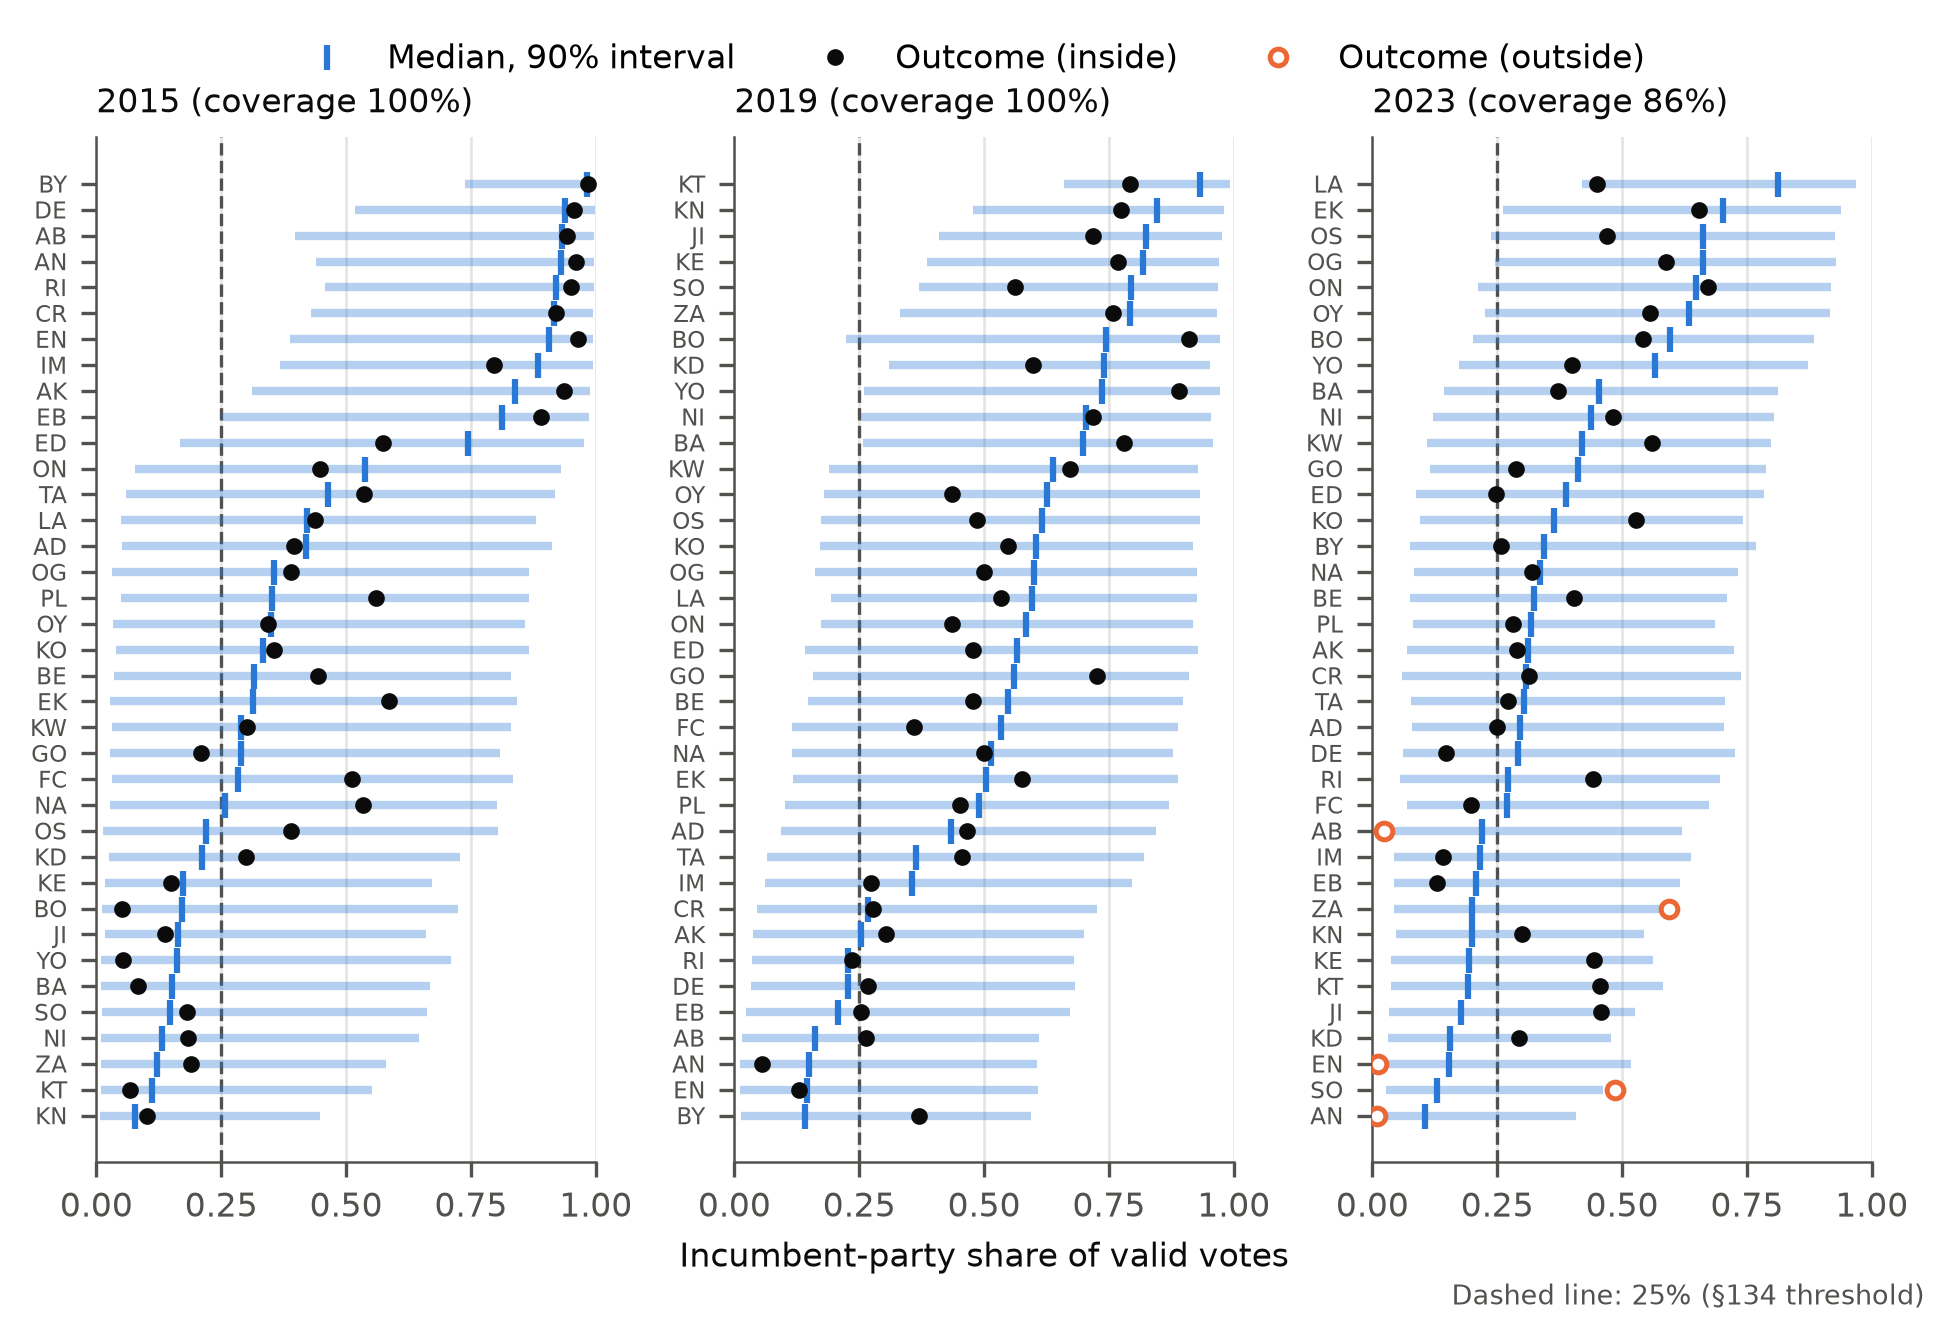
\includegraphics[width=\linewidth]{figures/fig2_backtest_intervals.png}
\caption{Prequential stack, oracle mode: posterior median and 90\% interval of the incumbent-party share in each of the 37 units against the outcome, for 2015, 2019 and 2023 (coverage 100\%, 100\%, 86\%). Hollow orange markers are outcomes outside the interval. Dashed line: the 25\% \S134 threshold.}
\label{fig:backtest_intervals}
\end{figure}

\subsection{Exploratory: shared zone shocks}
\label{sec:zoneshock}
The diagnosis suggests that errors are shared within regions. We therefore added to \texttt{pp\_region} and \texttt{ps\_region} an election-specific shock shared by the states of each geopolitical zone, $\omega z_{\text{zone}(i),t}$ with $\omega \sim \text{HalfNormal}(0.3)$, and refitted the backtests (posterior mean $\omega$ 0.78--0.97 against $\sigma$ 0.66--0.94; maximum $\hat{R}$ 1.008, no divergences). The zone-shock version of \texttt{pp\_region} has the lowest oracle CRPS of any model (7.41), and the two zone-shock models have the only forecast-mode CRPS below every baseline (9.94 and 9.82 against 10.16 for additive uniform swing). The zone-shock \texttt{pp\_region}'s count distribution is wider (standard deviation 2.7--2.9 units) and its spread probabilities were 0.66, 0.97 and 0.44. Its 2023 regional bias was smaller (northern states $-6.2$, southern $+3.2$) but not removed. These models were specified after the outcomes were seen, so this is not evidence of skill; it is a hypothesis, which we test with a second pre-registered 2027 forecast (Section~\ref{sec:forecast}).

\section{The 2027 Pre-registered Forecasts}
\label{sec:forecast}

\subsection{Design}
\sloppy The primary forecast refits the stack's two non-negligible members, \texttt{pp\_region} (weight 0.812) and \texttt{ps\_region} (0.188), on all five elections with state results, for the election of 27 February 2027. Its files and SHA-256 hashes were pushed to a public repository on 23 November 2026 and archived with a DOI [to be added]. A script in the repository checks out the public commit into a clean working tree, rebuilds the data panel with the committed code, reruns the forecast and compares hashes; the panel and the forecast's state and conditional files are reproduced byte for byte (the summary file differs only in its issue timestamp). A second forecast (v3) changes one thing, adding the shared zone shock to both members with the same weights, under a separately dated protocol; the v2 forecast remains primary. The target is the APC's share of valid votes, assuming that the incumbent president (Tinubu, South-West) is the APC candidate. The forecasts do \emph{not} forecast the outright winner or a second election: a national plurality depends on how the opposition vote splits, and the opposition line-up was not settled when they were issued. Results are reported for each geopolitical zone the main challenger could come from, with no probabilities attached.

\subsection{Results}
In every scenario the primary forecast's median APC national share is about 0.324, with a 90\% interval of roughly 0.19 to 0.51 and a probability of a national majority of about 0.05 (Appendix~\ref{app:scenarios}). The median lies below APC's 2023 share of 0.366 although the incumbent is running, because the posterior mean of $\mu + \gamma$ is $-0.19$ on the logit scale, about 4 points: the four elections with a sitting president running include 2015, when the incumbent party lost 14 points. Under alternative national priors the median ranges from 0.309 to 0.328. The probability of meeting the \S134 spread under the default legal reading ranges from 0.238 to 0.288 across scenarios (v3: 0.262--0.310); it is 0.212--0.271 if only the 36 states count, 0.189--0.234 if 25 whole units are required, and 0.066--0.156 under the petitioners' 2023 reading.

The state forecasts imply that the 2023 realignment deepens (Figure~\ref{fig:2027_states}). Decomposing the dominant member's forecast (Appendix~\ref{app:decomp}), the covariate terms, mainly the candidate home-zone and home-region indicators, add about 1.0 to 1.4 on the logit scale to southern states (1.9 in Lagos, the candidate's home state) even though the candidate's region is unchanged since 2023, because with persistence $\phi \approx 0.52$ the level model treats the 2023 deviations as not yet at the equilibrium the covariates imply. APC is forecast to rise in Lagos from 0.450 to 0.637 and to fall in Borno from 0.542 to 0.230, in Kwara from 0.561 to 0.287 and in Zamfara from 0.593 to 0.382. This is the pattern the same model over-predicted in the 2023 backtest, and it is the forecast's main known risk.

Because the national vote is weakly predictable, the forecast is most usefully read conditional on the national share (Figure~\ref{fig:2027_spread}). In the pre-registered 5-point grid, the probability of meeting the spread is at most 0.01 at a 30\% national share, 0.13--0.25 at 35\%, 0.56--0.77 at 40\% and 0.88--0.98 at 45\% (v3: 0.02--0.03, 0.21--0.31, 0.58--0.72 and 0.85--0.94). At APC's 2023 level of 36--37\% the primary forecast gives 0.26--0.35 on average across scenarios; APC met the spread at that level in 2023, and the backtests suggest this is too low.

\begin{figure}[ht]
\centering
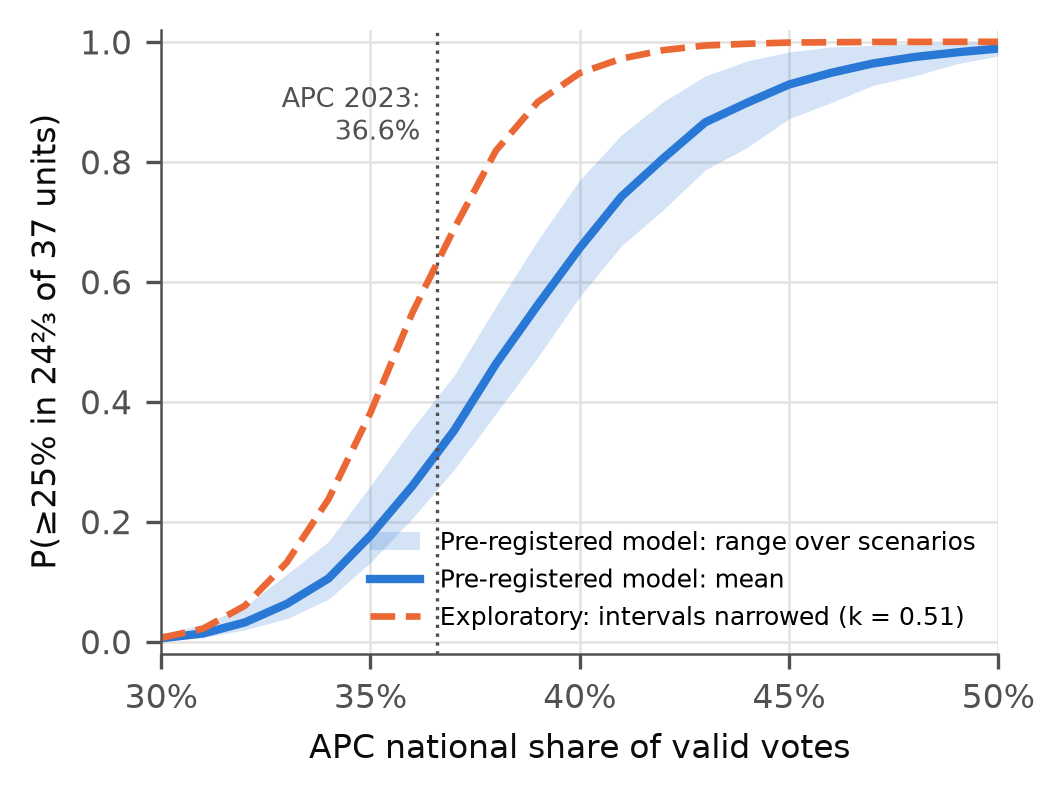
\includegraphics[width=0.75\linewidth]{figures/fig3_2027_spread_conditional.png}
\caption{2027 primary forecast: probability that APC obtains at least 25\% of the vote in $24\tfrac{2}{3}$ of the 37 units (\S134, default reading) as a function of APC's national share. Blue: the pre-registered model evaluated on a 1-point grid (values differ from the pre-registered 5-point file only by Monte Carlo error); line, mean over the six main-challenger scenarios; band, range. Dashed orange: exploratory variant with each state's predictive distribution narrowed by a factor of 0.51, not pre-registered. Dotted line: APC's 2023 national share (36.6\%).}
\label{fig:2027_spread}
\end{figure}

\begin{figure}[ht]
\centering
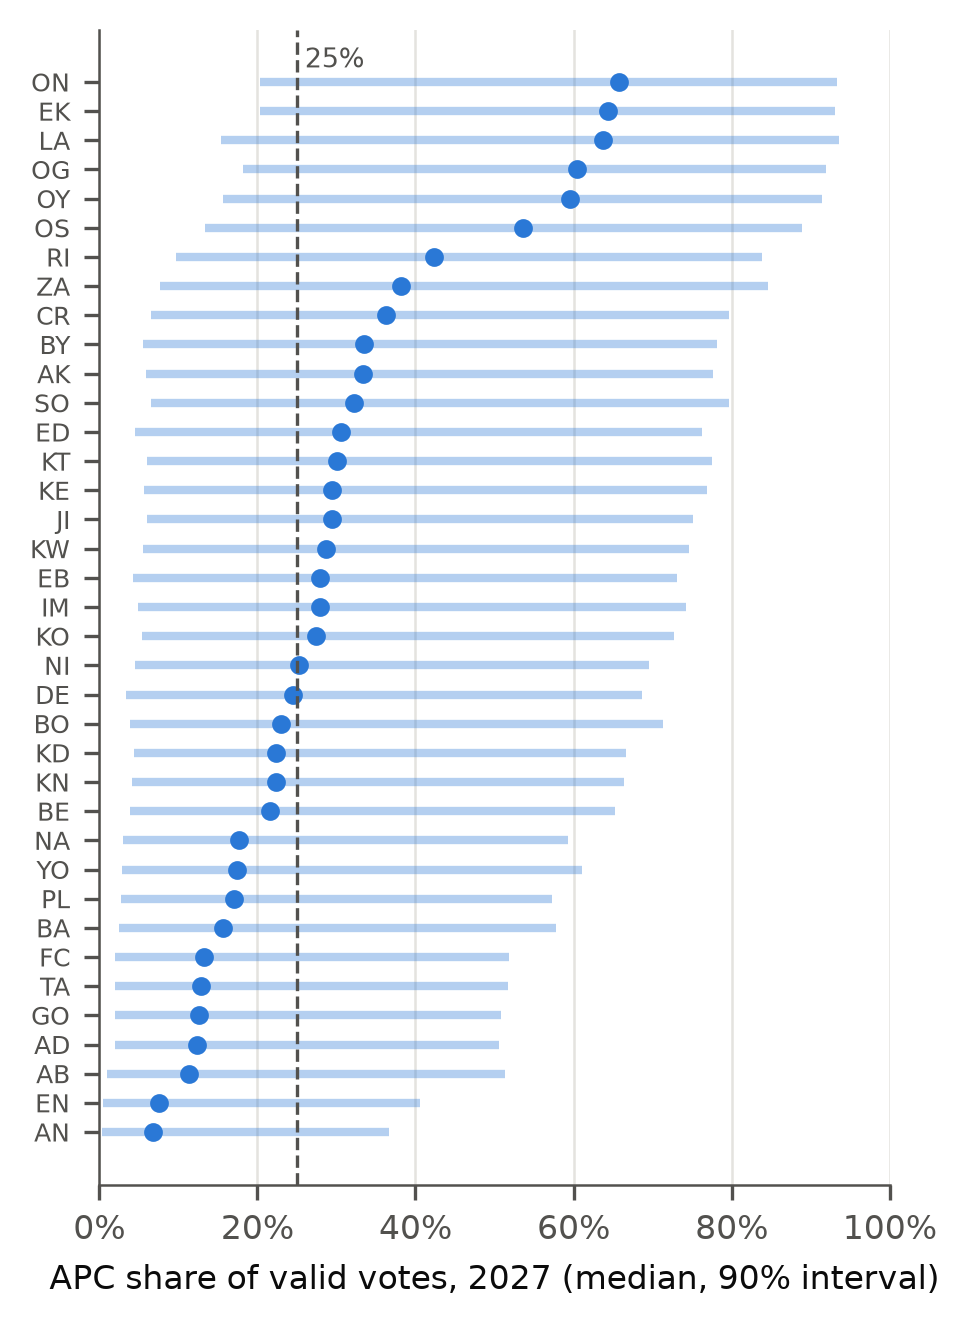
\includegraphics[width=0.6\linewidth]{figures/fig4_2027_states.png}
\caption{2027 primary forecast of APC's share of valid votes by state (posterior median and 90\% interval), scenario with the main challenger from the North-East. Dashed line: 25\% threshold.}
\label{fig:2027_states}
\end{figure}

\subsection{Evaluation rules}
An amendment to the pre-registration, made before the election and changing no forecast, fixes the evaluation. The scenario scored is that of the candidate whose party or coalition had the highest combined 2023 vote among the 2027 candidates (if this is indeterminate, that of the opposition candidate with the most 2027 votes, reported as outcome-informed), and all scenarios are also reported. The baselines are logit uniform swing, reconciled PUS and \texttt{ps\_null} fitted on all five elections, and a national no-change forecast of 36.6\%. The forecast will be judged to have shown state skill if its oracle-mode CRPS is below all three state baselines; national skill if its absolute national error is below the no-change error; and calibrated intervals if 30 to 36 of the 37 outcomes fall inside them. The spread probability is scored by the log score, in forecast mode against a climatological reference of 0.92 (the spread was met in all five elections with state results; $(5+\tfrac12)/(5+1)$) and in oracle mode at the true national share. Energy scores and the count RPS are also reported, and the primary and v3 forecasts are compared head to head. One election cannot settle any of these, and the results will be reported as such.

\fussy
\section{Discussion and Limitations}
\label{sec:discussion}
Four lessons follow, and they are mostly about what the historical record cannot do. First, the national vote is not forecastable from its own history: the national model does no better than a no-change forecast, and the largest recent swing coincided with a change in the number of serious candidates. Improving it requires information outside the series, such as the structure of the candidate field, cross-national evidence on incumbent-party swings, or polls, whose problems in Nigeria are well documented \citep{Mohammed2024OpinionPolls}. Any such extension should itself be pre-registered.

Second, threshold rules need multivariate evaluation. Unit-level intervals that are too wide coexisted with a count distribution that was too narrow, and the energy score and count RPS rank models differently from the CRPS (Tables~\ref{tab:results_oracle} and~\ref{tab:results_forecast}). In the simulation study, ignoring shared regional shocks leaves unit-level Brier scores unchanged but lowers the coverage of 90\% count intervals from 94\% to 88\%. The probability of the threshold event itself is driven mainly by where the units near the threshold sit, which is why the 2023 miss was a bias, not a dependence problem.

Third, few elections leave almost no power to compare state models. With three elections, even a model with a genuine state-level advantage is often ranked second, and forecast-mode reversals are expected by chance. We report score differences with block-bootstrap intervals and avoid claiming more than the data support. The same caution applies to stacking, whose weights from 37 to 111 correlated outcomes are noisy and which here amounted to model selection by 2023 \citep{Claeskens2016Puzzle}.

Fourth, the most promising improvement found, shared regional shocks, was found by looking at the outcomes. We therefore treat it as a hypothesis and test it with a second pre-registered forecast rather than reporting it as a result.

Further limitations remain. Five elections with state results inform the model, the 2015 backtest trains on two, and the 2003--2011 transition spans eight years. The backtests are only partly out of sample. Several elections were widely criticised by observers, and forensic analysis has suggested that vote counts in 2011 and 2015 deviate from patterns expected without manipulation \citep{Tunmibi2021MonteCarlo}, whereas our target is the declared result. The 2019 and 2023 state figures come from a secondary source, and candidate home states were coded from public information. The incumbent-running and incumbent-region effects are each identified by a single election. Finally, the forecasts do not model plurality against a fragmented opposition, which is likely to decide 2027.

\section{Conclusion}
\label{sec:conclusion}
We built a state-level results dataset for Nigeria's Fourth Republic, implemented the \S134 rule with its contested legal readings, and evaluated Bayesian state-level forecasts under a protocol designed to limit the overfitting that few elections invite. Given the national vote, the distribution of the vote across states is modestly forecastable; the national vote is not forecastable from the historical series; and the \S134 threshold count was poorly calibrated, for reasons that only a multivariate evaluation reveals. Two pre-registered 2027 forecasts, with evaluation rules fixed in advance, will provide a fully out-of-sample test.

\vspace{1em}
\noindent\textbf{Data and code availability.} Code, the curated results data, both evaluation protocols, all result files (including the exploratory analyses and the simulation study) and both pre-registered forecasts are available in a public repository [repository URL withheld for review]. ACLED's terms do not permit redistribution of its event data; the repository contains the derived state violence index and scripts that download the source data from the Humanitarian Data Exchange. Every number in this paper is produced by scripts in the repository.

\vspace{1em}
\noindent\textbf{Declaration of competing interest.} The author declares no competing interests.

\appendix

\section{Simulation study}
\label{app:simulation}
A synthetic country has 37 units in six zones of Nigeria's zone sizes and equal vote weights. In each election the true deviations are $d_i = \phi d^{\text{lag}}_i + \omega z_{\text{zone}(i)} + \sigma e_i$ with $\phi = 0.5$, $\omega = 0.8$ and $\sigma = 0.7$ (close to the fitted values of the zone-shock \texttt{pp\_region} model in the 2023 backtest), lagged deviations with variance 2 and a zone component, and outcomes reconciled to a national share drawn uniformly on $[0.35, 0.60]$. Predictive distributions use 400 draws.

\emph{Study 1 (power).} Forecaster A knows the data-generating process; forecaster B uses persistence $\phi_B \in \{1, 0.75, 0.625\}$ (1 is uniform swing) with noise matched to its residual variance. Both receive a national forecast with logit error of standard deviation $s$ and a calibrated predictive spread. Table~\ref{tab:sim1} reports how often A has the lower mean CRPS over three elections, in 300 replications per cell. Predictive draws are generated independently in the two modes, so at $s = 0$, where the modes coincide in distribution, the differences between the oracle and forecast columns (up to 0.02 in shares and 0.01 in gains) show the Monte Carlo error.

\begin{table}[ht]
\centering
\caption{Simulation study 1: share of three-election comparisons in which the better state model has the lower mean CRPS, and its mean advantage (CRPS points), by the size of the skill gap and of the national forecast error.}
\label{tab:sim1}
\small
\begin{tabular}{lrrrrr}
\toprule
$\phi_B$ & $s$ & \multicolumn{2}{c}{A ranked first} & \multicolumn{2}{c}{A's CRPS gain} \\
 & & oracle & forecast & oracle & forecast \\
\midrule
1.000 & 0.00 & 0.96 & 0.97 & 1.46 & 1.46 \\
1.000 & 0.50 & 0.98 & 0.98 & 1.44 & 1.19 \\
1.000 & 0.75 & 0.96 & 0.95 & 1.44 & 1.03 \\
0.750 & 0.00 & 0.85 & 0.83 & 0.50 & 0.49 \\
0.750 & 0.50 & 0.82 & 0.81 & 0.46 & 0.39 \\
0.750 & 0.75 & 0.84 & 0.83 & 0.45 & 0.30 \\
0.625 & 0.00 & 0.67 & 0.68 & 0.13 & 0.14 \\
0.625 & 0.50 & 0.67 & 0.72 & 0.12 & 0.10 \\
0.625 & 0.75 & 0.71 & 0.69 & 0.15 & 0.11 \\
\bottomrule
\end{tabular}
\end{table}

\emph{Study 2 (threshold counts).} Given the true national share, drawn on $[0.30, 0.45]$, forecaster C knows the zone shock and forecaster D has the same marginal variance with independent unit errors. Over 3,000 replications both have the same unit-level Brier score for the 25\% event (0.182) and essentially the same Brier score for the event ``at least 25 units'' (0.133 against 0.134), but D's 90\% count intervals cover 88\% of outcomes against C's 94\%, and 17\% of D's count PIT values lie outside $[0.05, 0.95]$ against 9\% for C.

\section{Count calibration and PIT histograms}
\label{app:count}

\begin{table}[ht]
\centering
\caption{Oracle mode: PIT of the outcome in the predictive distribution of the number of units at 25\%, and that distribution's standard deviation (units), by backtest. Exploratory.}
\label{tab:count}
\small
\begin{tabular}{lcccccc}
\toprule
& \multicolumn{2}{c}{2015 (26 units)} & \multicolumn{2}{c}{2019 (34 units)} & \multicolumn{2}{c}{2023 (29 units)} \\
Model & PIT & s.d. & PIT & s.d. & PIT & s.d. \\
\midrule
stack & 0.83 & 2.5 & 0.98 & 2.5 & 1.00 & 2.1 \\
pp\_region & 0.69 & 2.0 & 0.97 & 2.3 & 1.00 & 2.1 \\
ps\_null & 0.97 & 1.9 & 1.00 & 1.6 & 1.00 & 2.2 \\
sar\_region & 0.93 & 2.3 & 1.00 & 2.6 & 1.00 & 2.5 \\
pp\_region + zone shock & 0.69 & 2.7 & 0.96 & 2.9 & 0.99 & 2.8 \\
\bottomrule
\end{tabular}
\end{table}

Pooled over the three backtests in oracle mode, the share of state PIT values in the lowest or highest decile is 6\% for the stack, 3\% for \texttt{ps\_null}, 11\% for \texttt{pp\_region} and 4\% for the zone-shock \texttt{pp\_region}, against 20\% for a calibrated forecast: the unit-level distributions are too wide.

\section{Scenario detail for the 2027 forecasts}
\label{app:scenarios}

\begin{table}[ht]
\centering
\setlength{\tabcolsep}{4pt}
\caption{2027 primary pre-registered forecast by the main challenger's home zone: APC national share and probability of meeting the \S134 spread (default reading); last column, the v3 (zone-shock) forecast, whose national distribution is identical.}
\label{tab:2027_scenarios}
\small
\begin{tabular}{lrcrrr}
\toprule
Challenger zone & Median & 90\% interval & P($>$50\%) & P(spread) & v3 \\
\midrule
North-Central & 0.324 & [0.188, 0.508] & 0.055 & 0.246 & 0.275 \\
North-East & 0.324 & [0.191, 0.506] & 0.053 & 0.249 & 0.270 \\
North-West & 0.325 & [0.192, 0.504] & 0.053 & 0.288 & 0.310 \\
South-East & 0.325 & [0.188, 0.507] & 0.054 & 0.264 & 0.277 \\
South-South & 0.325 & [0.188, 0.508] & 0.054 & 0.238 & 0.262 \\
South-West & 0.324 & [0.191, 0.508] & 0.054 & 0.281 & 0.295 \\
\bottomrule
\end{tabular}
\end{table}

\section{Decomposition of the 2027 state forecasts}
\label{app:decomp}

\begin{table}[ht]
\centering
\caption{Contributions to the change in logit share from 2023 to 2027 in the dominant member (\texttt{pp\_region}, posterior means, North-East challenger scenario), for selected states, and the primary forecast's median. ``All covariates'' sums the home-state, home-zone, home-region and violence terms (current and lagged). The national swing ($-0.19$) and the intercept and state term (about $-0.28$) are similar for all states; the reconciliation shift is $-0.21$.}
\label{tab:decomp}
\small
\begin{tabular}{lrrrr}
\toprule
State & 2023 share & Mean reversion & All covariates & 2027 median \\
\midrule
Lagos & 0.450 & $-0.17$ & $+1.94$ & 0.637 \\
Ondo & 0.671 & $-0.60$ & $+1.42$ & 0.657 \\
Rivers & 0.442 & $-0.15$ & $+0.98$ & 0.423 \\
Kano & 0.299 & $+0.14$ & $+0.18$ & 0.223 \\
Borno & 0.542 & $-0.34$ & $-0.38$ & 0.230 \\
Kwara & 0.561 & $-0.38$ & $-0.05$ & 0.287 \\
Zamfara & 0.593 & $-0.44$ & $+0.20$ & 0.382 \\
Anambra & 0.008 & $+2.01$ & $+1.22$ & 0.068 \\
\bottomrule
\end{tabular}
\end{table}

\section{National model: prior sensitivity}
\label{app:national}

\begin{table}[ht]
\centering
\caption{National forecasts under alternative priors (exploratory). Baseline: $\mu,\gamma \sim \mathcal{N}(0,0.5^2)$, $\sigma_n \sim \text{HalfNormal}(0.5)$; the other rows change the scales as stated. Backtest columns: error of the median (percentage points), $\ast$ marking an outcome outside the 90\% interval. 2027: median and 90\% interval of APC's national share. $\gamma$: posterior mean (s.d.) when fitted on all five elections.}
\label{tab:prior_sens}
\small
\setlength{\tabcolsep}{4pt}
\begin{tabular}{lrrrcr}
\toprule
Priors & 2015 & 2019 & 2023 & 2027 & $\gamma$ \\
\midrule
Baseline (scales 0.5) & $+11.9$ & $-7.2$ & $+16.8$ & 0.324 [0.188, 0.508] & 0.25 (0.30) \\
Tight (scales 0.25) & $+12.0^\ast$ & $-7.0$ & $+17.2^\ast$ & 0.323 [0.204, 0.479] & 0.07 (0.19) \\
Wide (scales 1.0) & $+11.9$ & $-7.5$ & $+16.8$ & 0.328 [0.177, 0.524] & 0.43 (0.39) \\
$\sigma_n$ scale 1.0 & $+12.0$ & $-7.2$ & $+16.7$ & 0.325 [0.172, 0.525] & 0.23 (0.31) \\
No $\gamma$ & $+12.0$ & $-6.8$ & $+15.2$ & 0.309 [0.169, 0.500] & -- \\
\bottomrule
\end{tabular}
\end{table}

The posterior standard deviation of $\gamma$ is 60--75\% of its prior standard deviation under the baseline and tight priors and 39\% under the wide prior, so the single 2023 observation moves $\gamma$ only partly away from its prior.

\section{Stacking weights: robustness and uncertainty}
\label{app:weights}

\begin{table}[ht]
\centering
\caption{Weight of \texttt{pp\_region} (the remainder goes almost entirely to \texttt{ps\_region}; the other four candidates receive zero weight in the first three rows and have a resampled 95th-percentile weight of zero) under alternative density choices, and its sampling distribution from 200 resamples of states within each backtest. Exploratory.}
\label{tab:weights_robust}
\small
\begin{tabular}{lrrr}
\toprule
Densities & 2019 & 2023 & 2027 \\
\midrule
Gaussian, oracle (of record) & 0.700 & 1.000 & 0.812 \\
Gaussian, forecast mode & 0.840 & 1.000 & 0.745 \\
Kernel density, oracle & 0.601 & 1.000 & 0.793 \\
Resampled: median & 0.73 & 1.00 & 0.82 \\
Resampled: 90\% interval & [0.06, 1.00] & [0.82, 1.00] & [0.56, 1.00] \\
Resampled: share $> 0.5$ & 0.74 & 1.00 & 0.97 \\
\bottomrule
\end{tabular}
\end{table}

Choosing the weights from forecast-mode densities gives a stack with mean forecast-mode CRPS 10.65 against 10.66.

\section{Simulation-based calibration}
\label{app:sbc}
We checked the national model and the stack's dominant state model (\texttt{pp\_region}) by simulation-based calibration \citep{Talts2018SBC}. In each of 100 replications, parameters were drawn from the prior, data were simulated on the real design of the 2023 backtest (four training elections, the region covariates and the observed lagged deviations), the model was refitted (two chains of 500 draws after 500 tuning steps), and the rank of the true value among 99 thinned posterior draws was recorded. Table~\ref{tab:sbc} reports a $\chi^2$ test of uniformity over ten bins; no parameter shows a detectable departure, and no replication had divergent transitions. With 100 replications the test can detect only gross miscalibration.

\begin{table}[ht]
\centering
\caption{Simulation-based calibration: $p$-values of $\chi^2$ tests that the rank statistics are uniform (100 replications, 10 bins).}
\label{tab:sbc}
\small
\begin{tabular}{llr}
\toprule
Model & Parameter & $p$ \\
\midrule
National & $\mu$ & 0.83 \\
National & $\gamma$ & 0.70 \\
National & $\sigma_n$ & 0.76 \\
State (\texttt{pp\_region}) & $\alpha$ & 0.22 \\
State (\texttt{pp\_region}) & $\phi$ & 0.09 \\
State (\texttt{pp\_region}) & $\tau$ & 0.55 \\
State (\texttt{pp\_region}) & $\sigma$ & 0.14 \\
State (\texttt{pp\_region}) & $\beta$, incumbent home region & 0.51 \\
State (\texttt{pp\_region}) & $\beta$, challenger home region & 0.22 \\
\bottomrule
\end{tabular}
\end{table}

\bibliographystyle{elsarticle-harv}
\bibliography{references}

\end{document}
